\subsection{Metal Bare}
برای شروع تست در ابتدا
\lr{PostgreSQL}
را ری استارت می‌کنیم که تمام بافر‌ها را پاک کنیم. سپس
\lr{HammerDB}
را باز می‌کنیم. تعداد
\lr{warehouse}ها
را بر روی 16 و تعداد
\lr{user}ها
را بر روی 2 تنظیم می‌کنیم. در حین ساخت
\lr{schema}
نیز تمامی
\lr{syscall}ها و \lr{TLB event}ها
را زیر نظر می‌گیریم. به کمک دستورات زیر می‌توان این کار را انجام داد:
\codebox{
    perf record -p \$(pidof postgres | tr ' ' ',') -o hammerdb-schema-build-bare-metal-5.perf -e tlb:tlb\_flush,dTLB-loads,dTLB-load-misses,iTLB-load-misses,cache-misses,page-faults\\
    strace -f -p "\$(pidof postgres)" 2> hammerdb-schema-build-bare-metal-5.strace
}
کارکرد
\lr{HammerDB}
در زمان ساخت را می‌توانید در شکل
\ref{fig:postgres:baremetal:database:creation}
و سایز دیتابیس بعد از ساخت داده‌های
\lr{mock}
را می‌توانید در شکل
\ref{fig:postgres:baremetal:database:created}
ببینید.
\begin{figure}[H]
    \centering
    \subfloat{{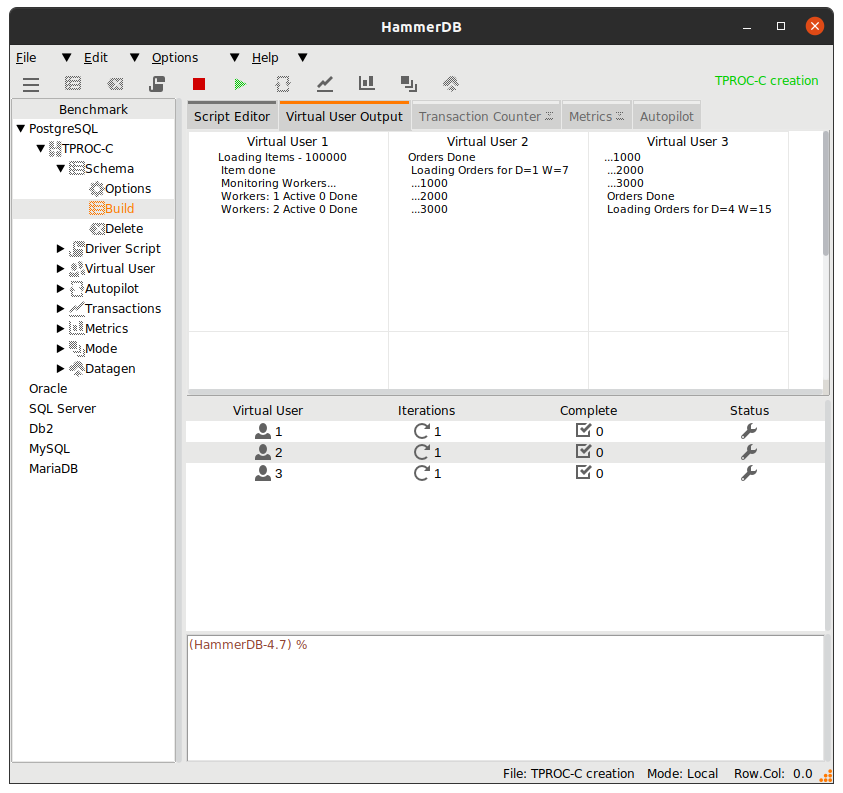
\includegraphics[scale=0.2]{pictures/postgres/baremetal/database-creation-1.png}}}
    \quad
    \subfloat{{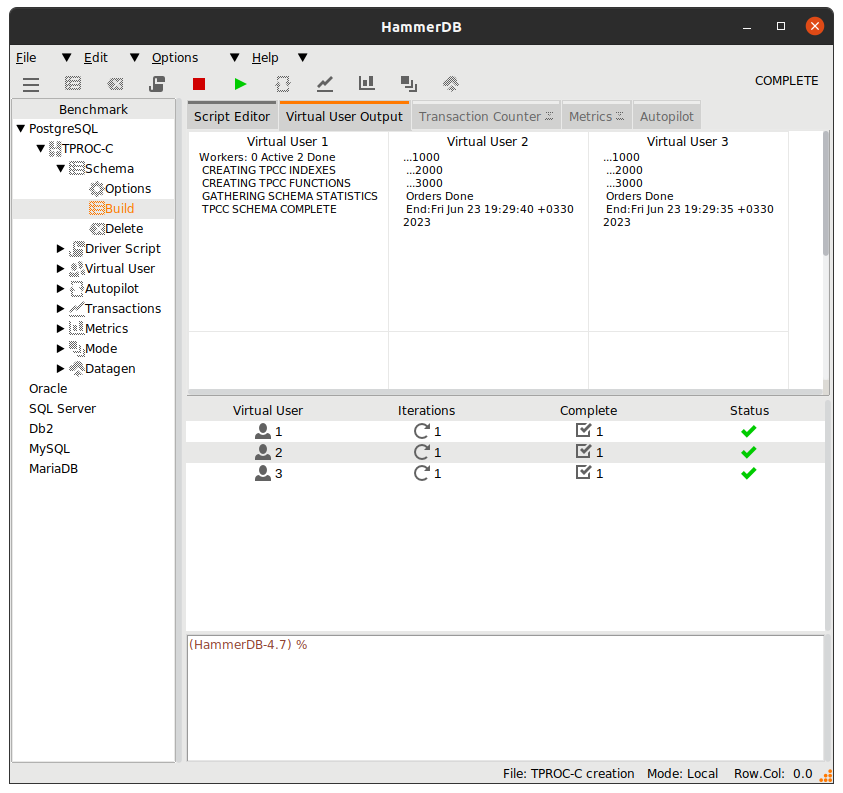
\includegraphics[scale=0.2]{pictures/postgres/baremetal/database-creation-2.png}}}
    \caption{ساخت \lr{schema}}
    \label{fig:postgres:baremetal:database:creation}
\end{figure}
\begin{figure}[H]
    \centering
    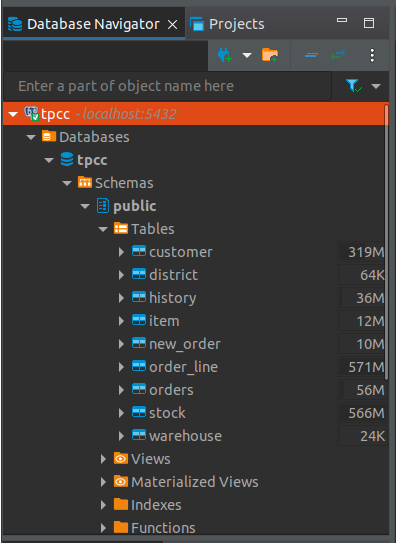
\includegraphics[scale=0.3]{pictures/postgres/baremetal/database-created.png}
    \caption{دیتابیس در \lr{DBeaver}}
    \label{fig:postgres:baremetal:database:created}
\end{figure}
در ادامه باید درایور را تنظیم کنیم. ما 3 دقیقه
\lr{rampup}
و 7 دقیقه
\lr{test}
را تنظیم کردیم. حال در ابتدا از قسمت
\lr{Transactions}، \lr{transactions meter}
را باز می‌کنیم که سرعت دیتابیس را بررسی کنیم. در نهایت در قسمت
\lr{virtual users}
بر روی
\lr{Create} و \lr{Run}
کلیک می‌کنیم. با این کار تست شروع می‌شود. عکس‌های مربوط به تست را می‌توانید در عکس
\ref{fig:postgres:baremetal:database:benchmark}
مشاهده کنید.
\begin{figure}[H]
    \centering
    \subfloat[\centering در حال اجرا]{{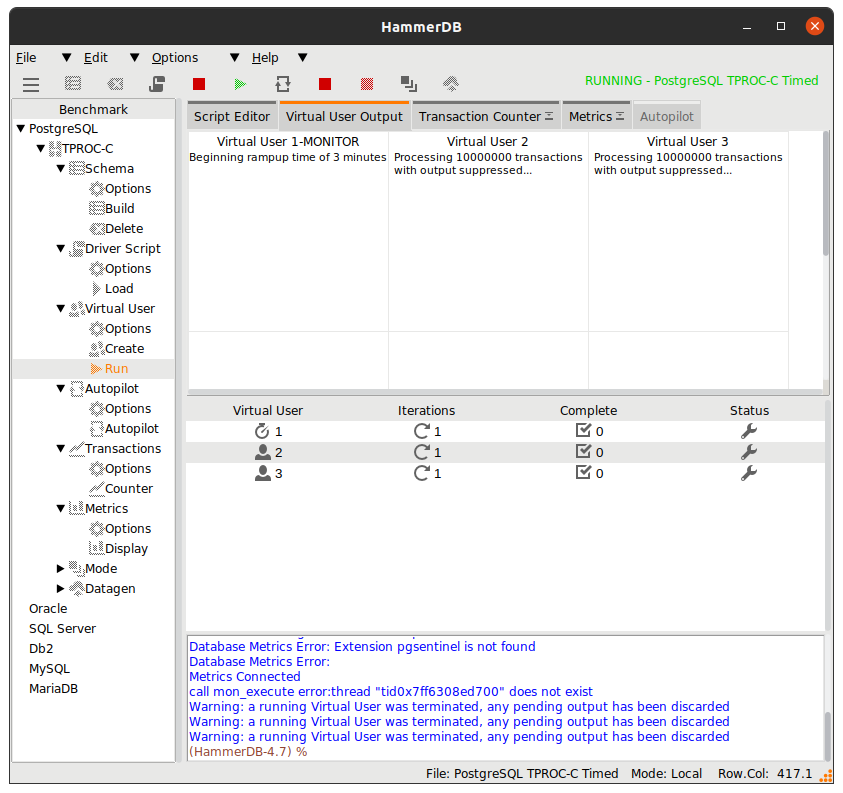
\includegraphics[scale=0.2]{pictures/postgres/baremetal/run.png}}}
    \quad
    \subfloat[\centering TPM در ابتدا]{{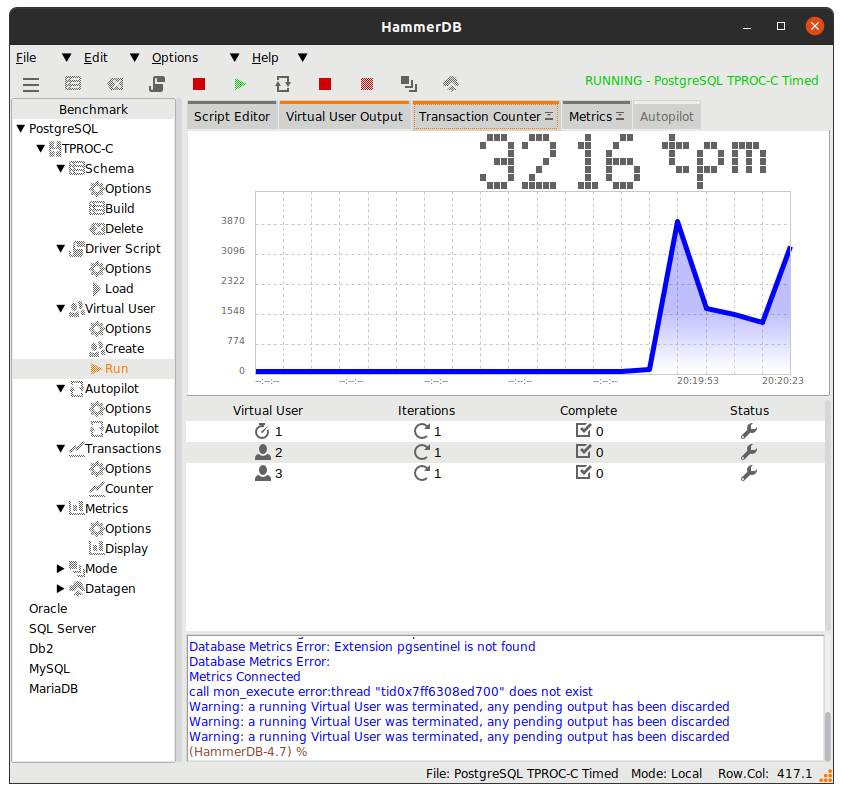
\includegraphics[scale=0.2]{pictures/postgres/baremetal/tpm1.png}}}
    \quad
    \subfloat[\centering TPM در انتها]{{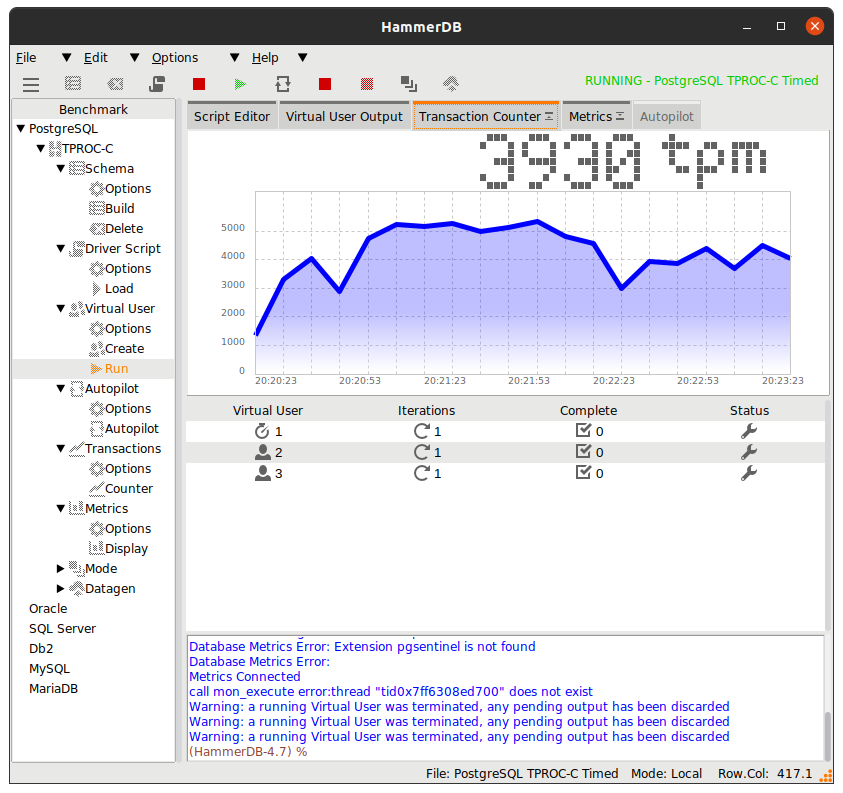
\includegraphics[scale=0.2]{pictures/postgres/baremetal/tpm2.png}}}
    \quad
    \subfloat[\centering پایان بنچمارک]{{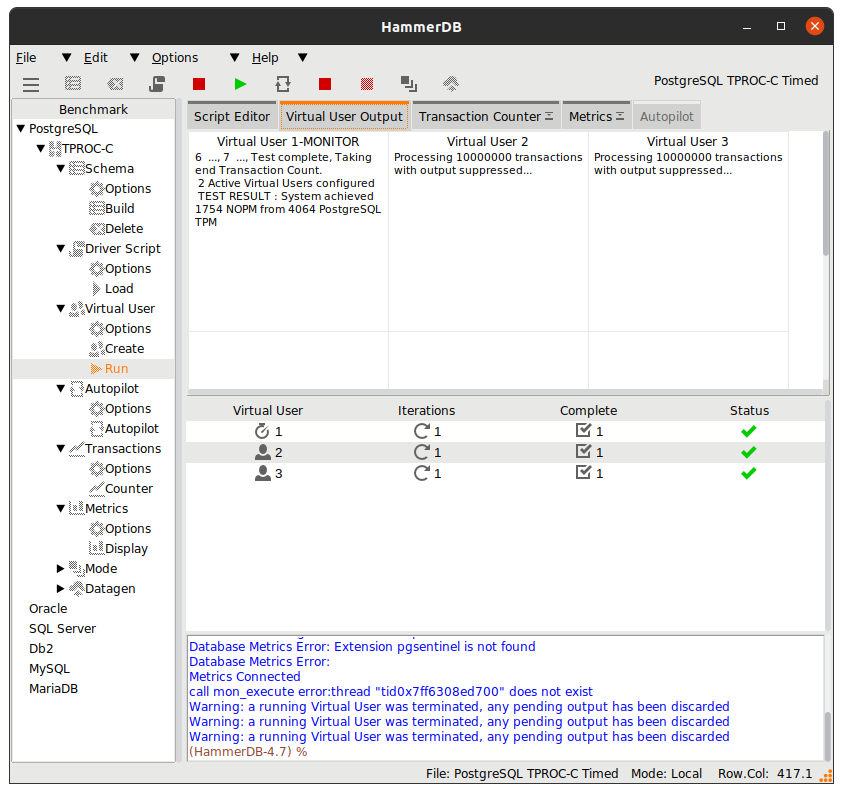
\includegraphics[scale=0.2]{pictures/postgres/baremetal/done.png}}}
    \quad
    \subfloat[\centering btop]{{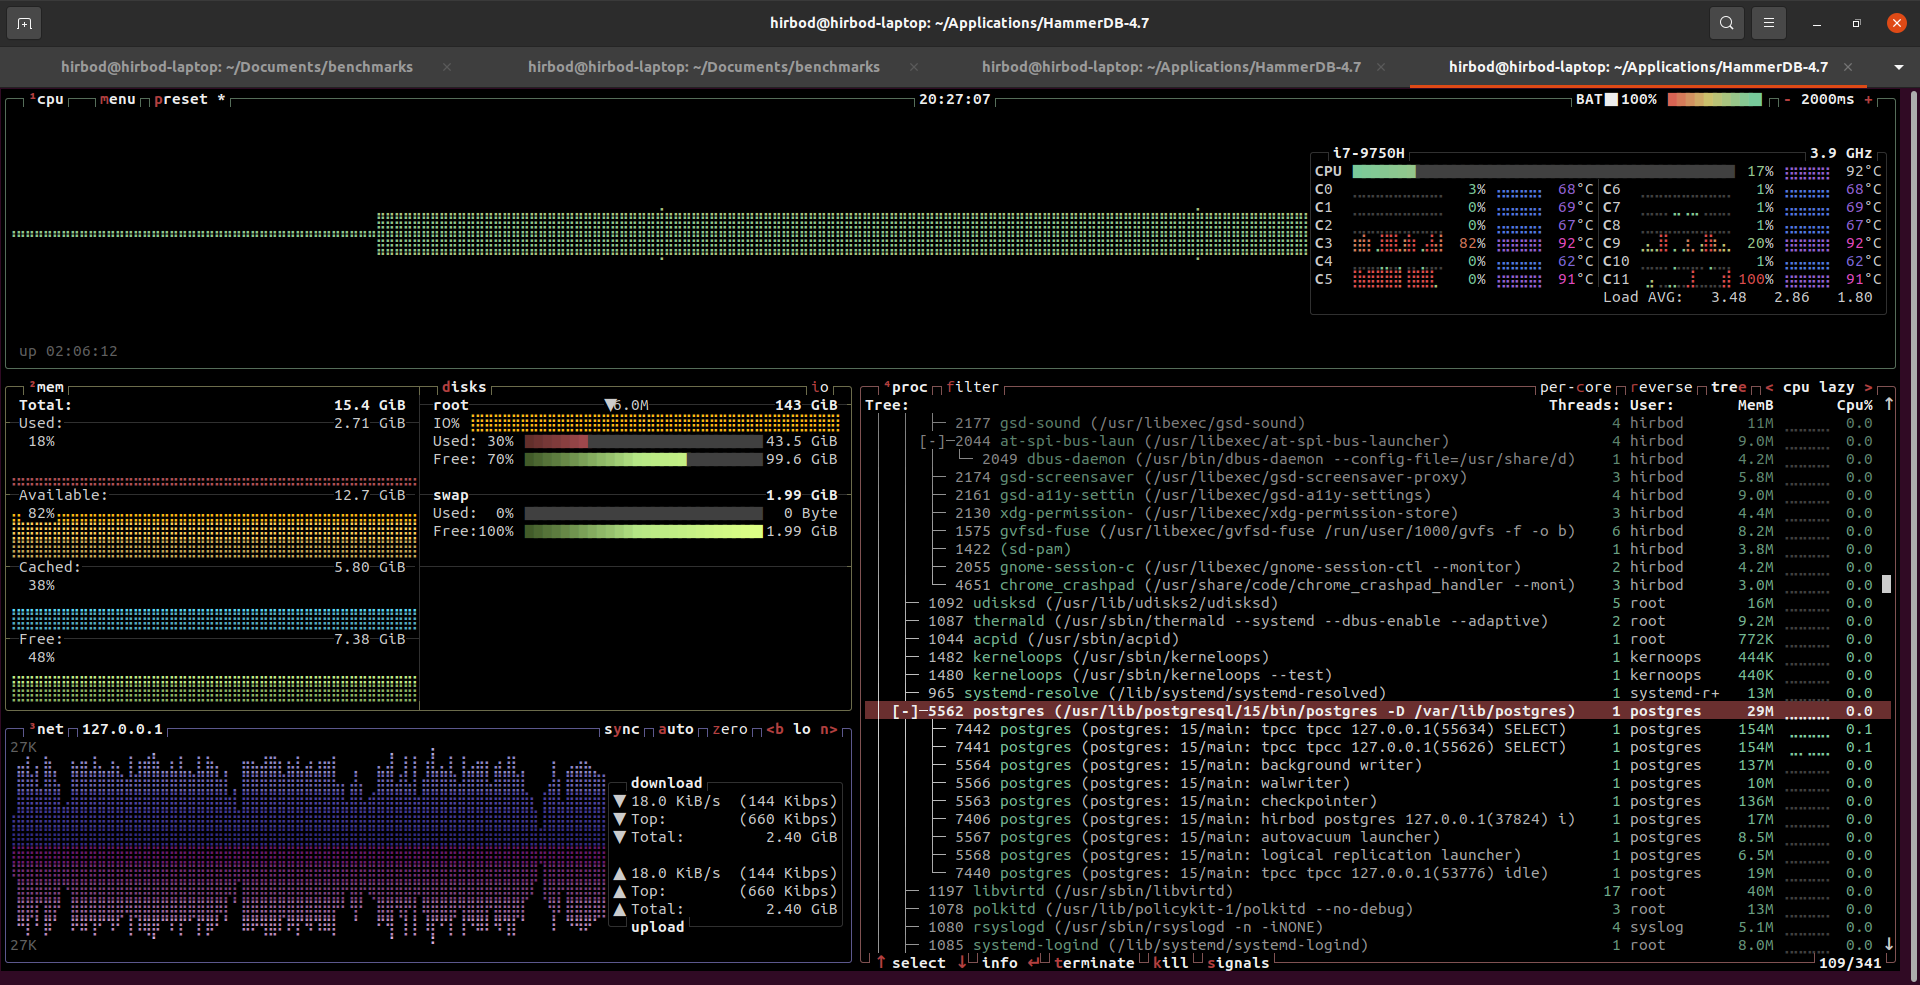
\includegraphics[scale=0.2]{pictures/postgres/baremetal/btop.png}}}
    \caption{دیتابیس در حال بنچمارک شدن}
    \label{fig:postgres:baremetal:database:benchmark}
\end{figure}

\smalltitle{مشکل کرنل 3}
یکی از مشکلات بسیار عجیبی که به آن در تست‌هایمان بر خوردیم این بود که اجرای
\lr{HammerDB}
بر روی کرنل 5 باعث کرش کردن
\lr{display manager}
می‌شد! یعنی کل
\lr{session}
من پاک می‌شد و به صفحه‌ی
\lr{login}
منقل می‌شدم. به همین دلیل از تست کردن
\lr{PostgreSQL} و \lr{MySQL}
بر روی کرنل نسخه‌ی 3 منصرف شدیم.
